\chapter{Response generation}

This chapter mainly details the functionality and implementation of the response generation component. As emphasized in sections [SECTION], [SECTION], response generation depends on the outputs of the information extraction, classification, and identity generation components. 

We begin by briefly introducing the identity generation component. We continue with the bucketing algorithm for grouping messages into conversation threads. Next, we discuss strategies for generating engaging replies. In section [SECTION], we go into detail on how responses are generated and provide examples. Finally, in [SECTION], we outline briefly the mechanism to send out emails anonymously.

\section{Identity generation}
The purpose of the identity generation component is to provide our agent with a consistent persona. This is accomplished by attaching an identity to each conversation thread. An identity consists of the following information: \textit{name, age, occupation, email address, postal address, country, marital status}, which we have determined to be frequently requested by advance fee fraud scammers ([Background]). This information is fictitious and may be given out by the response generation component, based on the current conversation state and strategy. As the available time for this project is limited, our prototype implementation of this component only provides middleware functionality, as well as a bank of five manually compiled identities. Therefore, a possible extension over this project is to provide the functionality to randomly generate new identities on the fly.

\section{Bucketing algorithm}
The first step in generating a response to an incoming message is to determine whether the message belongs to a conversation thread. We define a thread as a logical unit of all messages related to a single instance of a scam. Furthermore, it is important to note that a single instance may involve multiple actors [SECTION, Background]. Formally, given an incoming message $M$ and a set of threads $T = $\{$T_{1}, T_{2}, ..., T_{n}$\}, determine if $\exists M \in T$.
	
This is a challenging problem. A na\"{\i}ve approach assumes that each conversation thread can contain at most two actors -- the agent and the scammer. Therefore, keeping track of the \emph{From} header is  sufficient to maintain conversation state. Another approach is to compute the thread with the largest word overlap for each incoming message. This is a better solution, but it makes the assumption that the message body always contains a quoted response. Due to the nature of AFF scams, this is also ineffective.

We propose a bucketing algorithm which combines ideas from the aforementioned approaches with one important observation -- the scammer always notifies the target in advance when he is being transferred to a third party -- e.g. ``\textit{please contact the prize remittance manager, John Smith at john.smith@domain.com}''. Therefore, an effective way to keep track of threads is to keep track of the mentioned emails in each message. In order to do this, we attach a bucket to each thread that collects all email addresses. Once a new message comes in, we try to match it to a bucket. If successful, we update the bucket with any new email addresses. Otherwise, we create a new thread.

For example, let us assume we have threads $T_{1}, T_{2}, T_{3}$ with corresponding buckets $B_{1}, B_{2}, B_{3}$, such that $B_{1} = $\{$E_{1}, E_{2}$\}, $B_{2} = $\{$E_{3}$\}, $B_{3} = $\{$E_{5}$\} where $E_{n}$ is an email address. Message $M_{1}$ enters the system with a candidate bucket $B_{c} = $\{$E_{3}, E_{6}$\}. Then, for $B_{n}$ in $B$, $\operatorname{arg\,max} \left|{B_{n} \cup B_{c}}\right| = $\{$1$\}. Therefore, we attach $M_{1}$ to $T_{2}$ and update $B_{2} \coloneqq B_{2} \cup B_{c}$. Message $M_{2}$ enters the system with a candidate bucket $B_{c} = $\{$E_{10}$\}. For $B_{n}$ in $B$, $\operatorname{arg\,max} \left|{B_{n} \cup B_{c}}\right| = $\{$0$\}. Therefore, we create a new thread $T_{4}$ with $B_{4} \coloneqq B_{c} \cup \emptyset$.

\section{Strategies}
The agent employs a set of strategies designed to occupy the scammer for as long as possible. These strategies can be divided into two categories -- cooperative and non-cooperative. Cooperative strategies are mainly used to gain the scammer's confidence and are fulfilled by responding positively to requests. Non-cooperative strategies are used throughout each conversation thread and aim to deflect questions, drive the conversation to a different topic, or elicit extra work from the scammer.

\subsection{Cooperative strategies}
In our implementation, we use three different cooperative strategies. The first strategy is to always express interest in any proposed scheme in the beginning of a conversation thread. The initial responses are always enthusiastic and reaffirm the premise set up by the scammer. For example, if the scammer's initial email claims we have won the lottery, we do our best to pretend that we did. This strategy helps create the impression that the agent is a viable target and encourages the scammer to spend time replying back.

Another cooperative strategy involves responding to requests for personal information . As we discussed in [CHAPTER], scammers commonly request personal information as a way to establish the target's trust. If the target gives out personal details, it is considered much more valuable to the scammer, as it is very likely to cooperate with other future requests. Therefore, a useful strategy for our agent is to respond positively to these requests. If asked, our agent responds to these requests with personal details obtained from the identity generation component. This helps build up the scammer's perception that the agent is a viable target and makes him more invested in the conversation.

The final cooperative strategy is reaffirmation. Reaffirmation is used throughout each conversation thread to restate the agent's interest in the scammer's proposition. It is often used in conjunction with non-cooperative strategies to express that we are still interested in the scheme, despite any setbacks we might have introduced. For example, an example of reaffirmation is claiming -- ``\textit{I look forward to working with you to process my winning}'' at the end of the message, whilst asking many extra questions in the message body.

\subsection{Non-cooperative strategies}
We use four main non-cooperative strategies in the implementation of our agent. The first non-cooperative strategy is deflecting questions. As we discussed in [SECTION], answering certain types of questions is beneficial, as it helps establish trust. However, complying with other types of questions can be dangerous or impossible. One example are requests for photo identification. Cooperating with these is clearly a bad idea. Instead, we choose to compose excuses -- e.g. ``\textit{I am sorry, but I am bad with computers. Could you tell me how to put a photo in this letter?}'' Excuses are usually effective at bypassing these questions altogether. Alternatively, the scammer has to spend the time to write a mini tutorial on how to work with email attachments. 

Another non-cooperative strategy is asking questions about exceptional circumstances. As we observe in [SECTION], answering questions is a challenging NLP task. Instead, it is better to ask questions and attempt to drive the conversation. These questions are closely related to the variation of the scam in play and are designed to elicit extra work from the scammer. For example, in the context of a lottery scam, the agent might ask if the winnings are subject to any tax or whether they can be paid out in Australian dollars.

Stories are the third non-cooperative strategy. They are employed in later stages of a conversation and are context independent. The main purpose of stories is to take up the scammer's time by having him read a large chunk of text, following a few initially promising exchanges. Because of this, each story is between 350 and 600 words long. At the end of a story, the scammer is asked whether he can relate to the situation described in the story. By requesting a comment, we validate that he has read the story.

Lastly, our final non-cooperative strategy is to prompt the scammer to resend messages. This behavior is elicited by composing replies that claim the scammer's previous message has been accidentally deleted, is garbled, or has never been received. This strategy has a single goal -- to force the scammer to look through his inbox, find the correct message, and resend it. It is a simple way to get the scammer to do extra work.

\section{Composing a response}
Responses are generated from the outputs of the information extraction, identity generation, classification tasks and current conversation state via a multi-layer finite state machine. The process works as follows: the top layer FSM builds a template with placeholders for lower-level probabilistic finite state machines (PFSMs). The lower-level PFSMs emit text or another layer of PFSMs. At the bottom layer, all PFSMs generate text. This approach can also be described as top-down text generation.

\subsection{Understanding the context}
Understanding natural language is a very challenging task. Fortunately, advance fee fraud scams tend to follow a set pattern within a relatively narrow domain ([CHAPTER]). This makes it possible for us to use techniques such as machine learning, pattern matching rules and the conversation state to generate convincing replies.

Two maximum entropy classifiers are central to our effort to understand the contents of an incoming message. The the scam type classifier helps determine which one of the 22 known AFF variations is currently in play. For example, if we are dealing with an instance of a lottery scam, we will use the corresponding lottery PFSMs and text snippets to generate that part of the response. The second classifier helps determine whether the scammer asks us to provide any personal information. If so, similarly as before, we will use another set of corresponding PFSMs to generate that information.

Rules are the second method we use to understand the context of a message. Rules are specific to each AFF variation and allow us to look for patterns that are strong signals for conversation state. In the aforementioned lottery scam, we recognize four distinct states -- \textit{initial, claim form approved, payment approved, fee request}. Knowing the current state allows us to generate a reply with information specific to that state and creates the impression of a natural response.

Finally, it is not always possible to understand the context of a message through a classifier or rules.
Where this is not possible, we use the current state of the thread, as determined by the bucketing algorithm, and compose a reply using a non-cooperative strategy. For example, if the current state shows we are in the beginning of a thread, we will use the asking questions PFSM. In later stages, we will pick randomly between prompting the scammer to resend the message or the story strategy.

\subsection{Text snippets}

We use text snippets in the final states of the PFSMs to generate large paragraphs of text. These text snippets are written ahead of time and are stored in a hierarchical tree data structure. Top-level nodes represent specific scenarios -- “\textit{photo request}”, “\textit{lottery}”, etc. Scenarios which describe scam variations have another set of mid-level nodes which list all recognized states of the variation. Finally, at the bottom of the tree, leaves contain a set of text snippets associated with their parent nodes. Text snippets are diverse, but usually consist of 1--3 sentences, with placeholder variables for conversation-specific information (e.g. the agent's identity). For the current system prototype, we have defined 37 nodes and 169 text snippets. Extending the collection of text snippets is easy and requires no changes to the implementation -- new snippets can be saved as text files in the file system.

Further to adding context, text snippets also provide variability to the generated responses. This is accomplished through redundant tree leaves. These leaves have similar sentiment, but are phrased in different ways. Let us illustrate this. Consider the example scenario of answering questions for personal information. The response paragraph is constructed from text snippets of the following bottom-level tree nodes: intro, name, age, occupation, location, postcode, contact details, closing. These nodes have 5, 7, 8, 5, 4, 2, 6, 6 leaves respectively. A PFSM crawls the tree and randomly selects a single leaf from each parent node. The outputs are then compiled into the final text paragraph. In this instance, the aforementioned process allows for $8 \times 7 \times 6^2 \times 5 ^ 2 \times 4 \times 2 = 403,200$ distinct paragraph compositions. As such, the probability of generating a duplicate response is very low. We use this approach to generate each paragraph of the outgoing message.

\subsection{Finite state machines}

Several layers of FSMs and PFSMs determine how each response is generated. We start by looking at the top-level FSM. We move on to a simple PFSM used for generating greetings. Finally, we illustrate the PFSMs that generate the content body.

The top-level FSM defines the high-level structure of our message -- a letter. The Greeting, Body and Signature states represent a set of PFSMs, whilst Quoted\_Text simply produces a quoted version of the incoming message. The FSM is illustrated in [FIGURE].

\begin{figure}[h]
\centering

\includegraphics{pics/top-level-fsm.png}
\caption{The top-level FSM defines a letter structure for the message}
\end{figure}

The greeting generation automata is an example of a simple bottom-level PFSM. Its task is to accept the name of the scammer and produce a greeting, as illustrated in [FIGURE]. The transitions between the has\_name state and the text snippets have probability $p = \frac{1}{3}$.

\begin{figure}[h]
\centering
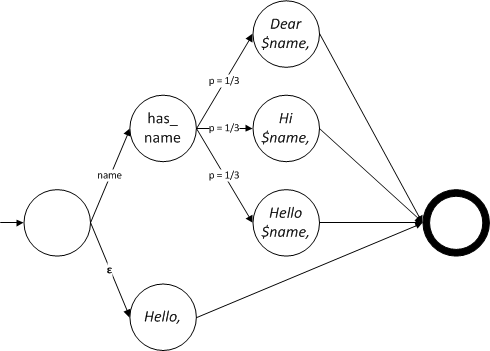
\includegraphics{pics/greeting-fsm.png}
\caption{The greeting generation PFSM}
\end{figure}

Figure 7.3 illustrates the PFSM which generates the content body of a message. It takes in as inputs the results of classifier, information extraction and identity generation tasks. Its main purpose is to select strategies and create placeholders for lower-level PFSMs. Strategies are selected based on the available information and conversation state. Please note, for clarify of the figure, we have omitted some of the notation.
\begin{figure}
\centering
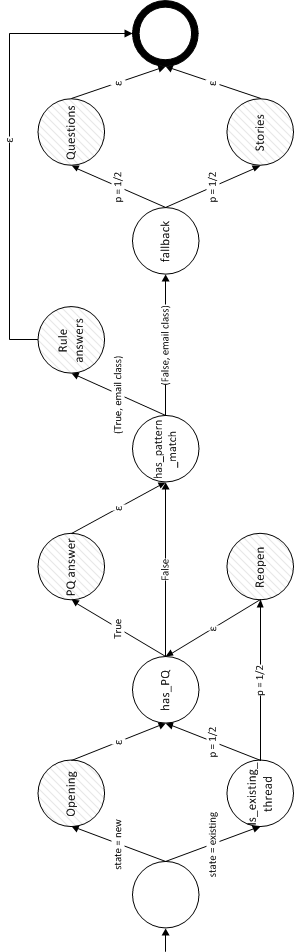
\includegraphics{pics/body-fsm-left.png}
\caption{This PFSM determines which strategies to include in the body of the message.}
\end{figure}

Figure 7.4 (a) illustrates a lower-level FSM which models a lottery scam. The scam has four distinct states. Figure 7.4 (b) illustrates a bottom-level PFSM for the same scam, after a successful transition to the initial state.

\begin{figure}[h]
  \centering
  \subfloat[Lottery scam model]{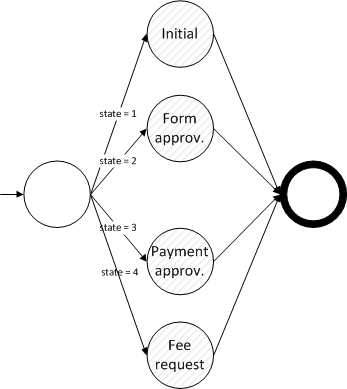
\includegraphics[scale=0.80]{pics/lottery-fsm.png}}
  ~ %add desired spacing between images, e. g. ~, \quad, \qquad etc. (or a blank line to force the subfig onto a new line)
  \subfloat[Text snippet PFSM]{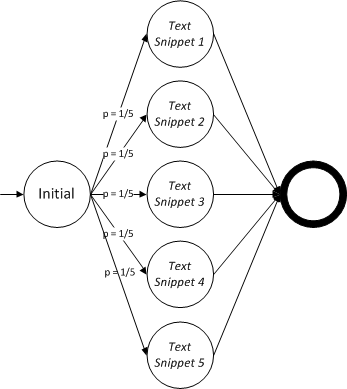
\includegraphics[scale=0.80]{pics/text_snippet_fsm.png}}
  ~ %add desired spacing between images, e. g. ~, \quad, \qquad etc. (or a blank line to force the subfig onto a new line)
%  \subfloat[A mouse]{\label{fig:mouse}\includegraphics[width=0.3\textwidth]{mouse}}
  \caption{A model of the lottery scam and text snippet selection for the \emph{Initial} state}
 % \label{fig:animals}
\end{figure}

We follow the same approach when modeling other scam variations and conversation strategies.

\clearpage
\subsection{An example message}
In Figure 7.5, we present a sample message annotated with colors.
\begin{itemize}
\item \textcolor{Red}{Red} denotes the outputs of the named-entity recognition and relation extraction tasks.
\item \textcolor{Green}{Green} denotes that the classifier has determined this message is an instance of the \textit{Orphans} class. The response generation component has appropriately selected the \textit{Orphans} PFSM and generated these sentences.
\item \textcolor{Yellow}{Yellow} is an example of an affirmative strategy -- reassuring the scammer that we will cooperate.
\item \textcolor{Blue}{Blue} illustrates the strategy of asking questions. Each question is generated separately by a PFSM from a bank of questions relevant to the scam class.
\item \textcolor{Brown}{Brown} shows the current identity of the agent for this thread.
\item \textcolor{CarnationPink}{Pink} is the scammer's original message, quoted and formatted in a similar style to Gmail.
\end{itemize}

\begin{figure}[h]
	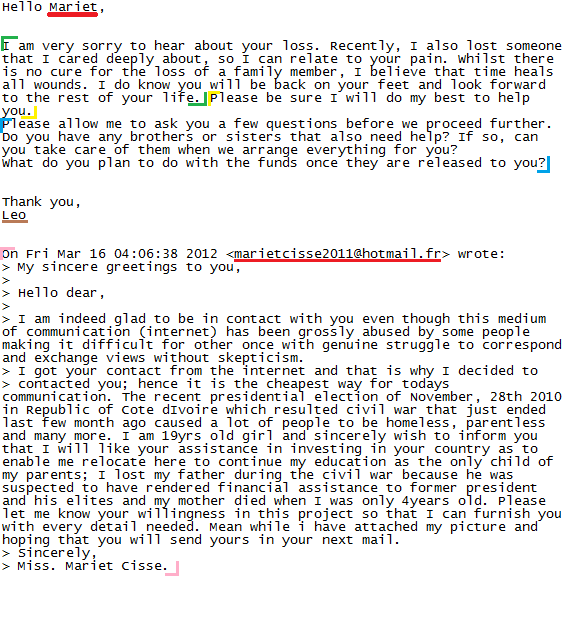
\includegraphics{letter.png}
	\caption{An example message generated by our system, annotated with colors. See Subsection 7.4.4. }
\end{figure}

\subsection{Sending the reply}
As we described in [SECTION], anonymous email accounts are used to send and receive emails. In order to ensure consistency, each thread has an associated identity and email account. Once a message is generated, it is transmitted via a SSL connection to the SMTP server

Through experimentation, we have established that sending 40 messages with less than a second delay between messages results in the termination of the associated email account by the provider. To mitigate this, we observe a random backoff period between consecutive SMTP connections. This is currently set to a minimum of 70 and a maximum of 170 seconds between connection attempts.
